\section{Exercise 1 - Mid-depth temperature and \delO{SW} reconstruction}

\begin{figure}
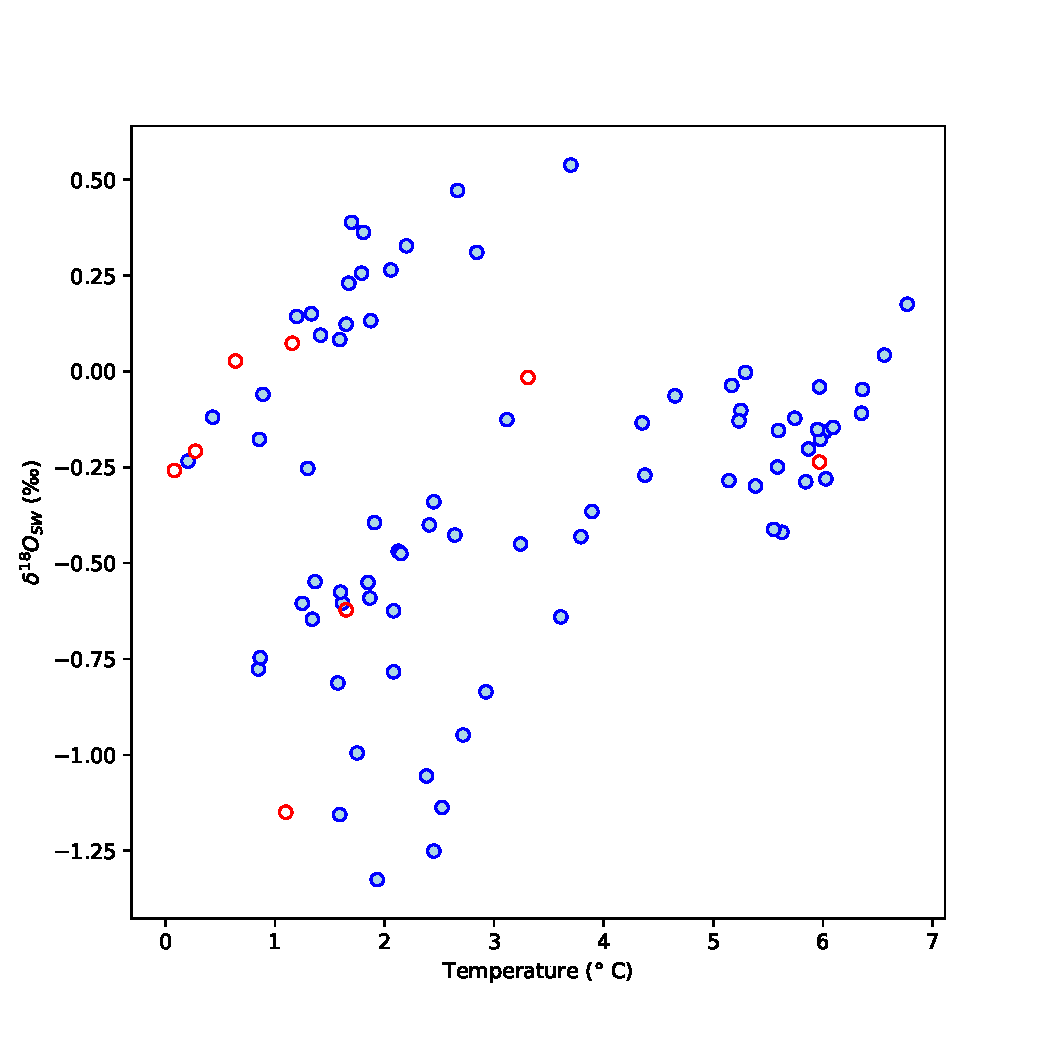
\includegraphics[width=\textwidth]{img/scatter_temp_x_d18Osw}
    \caption{Scatter plot of bottom water temperature from Mg/Ca palaeothermometry against ice volume corrected oxygen isotope excursion (\delO{SW}), both from benthic foraminifera M. barleeanuum.
             Red points mark measurements rejected for contamination.}
        \label{fig:tempxd18Osw}
\end{figure}

\begin{figure}
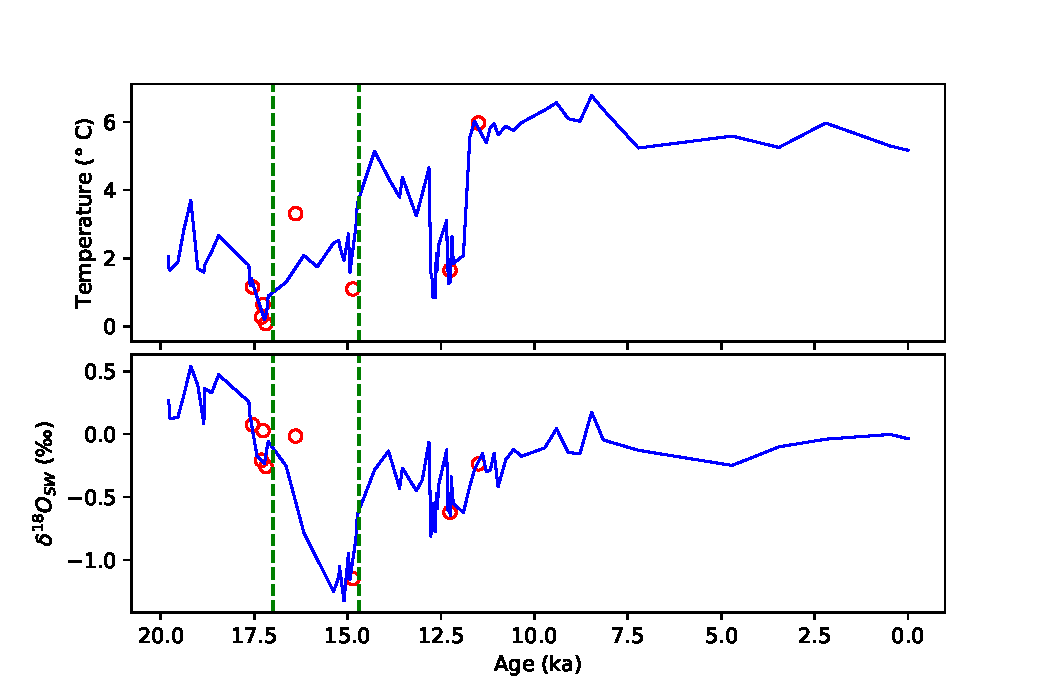
\includegraphics[width=\textwidth]{img/timeseries_temp_and_d18Osw}
    \caption{Time series of: bottom water temperature (top) and ice volume corrected oxygen isotope excursion (bottom).
             Dashed green lines indicate approximate boundaries of Heinrich Stadial, red points as in Figure \ref{fig:tempxd18Osw}}.
        \label{fig:timeseriestempd18Osw}
\end{figure}
